\chapter{Implementation}
\label{chap:implementation}

This chapter details the practical realization of the indoor localization system described in the previous sections. It covers the overall system architecture, the design and configuration of the ESP32 BLE beacons, the development of the smartphone application, and the integration of the MQTT broker for communication. Each component is discussed in terms of its role, implementation choices, and how they collectively contribute to a robust and scalable solution for museum environments.

\section{System Architecture}
The full system is composed of three different components, each playing a crucial role in its functionality. \autoref{fig:schema} illustrates the overall architecture of the system, highlighting the interactions between the ESP32 devices, the smartphone application, and the MQTT broker.

\begin{figure}
    \centering
    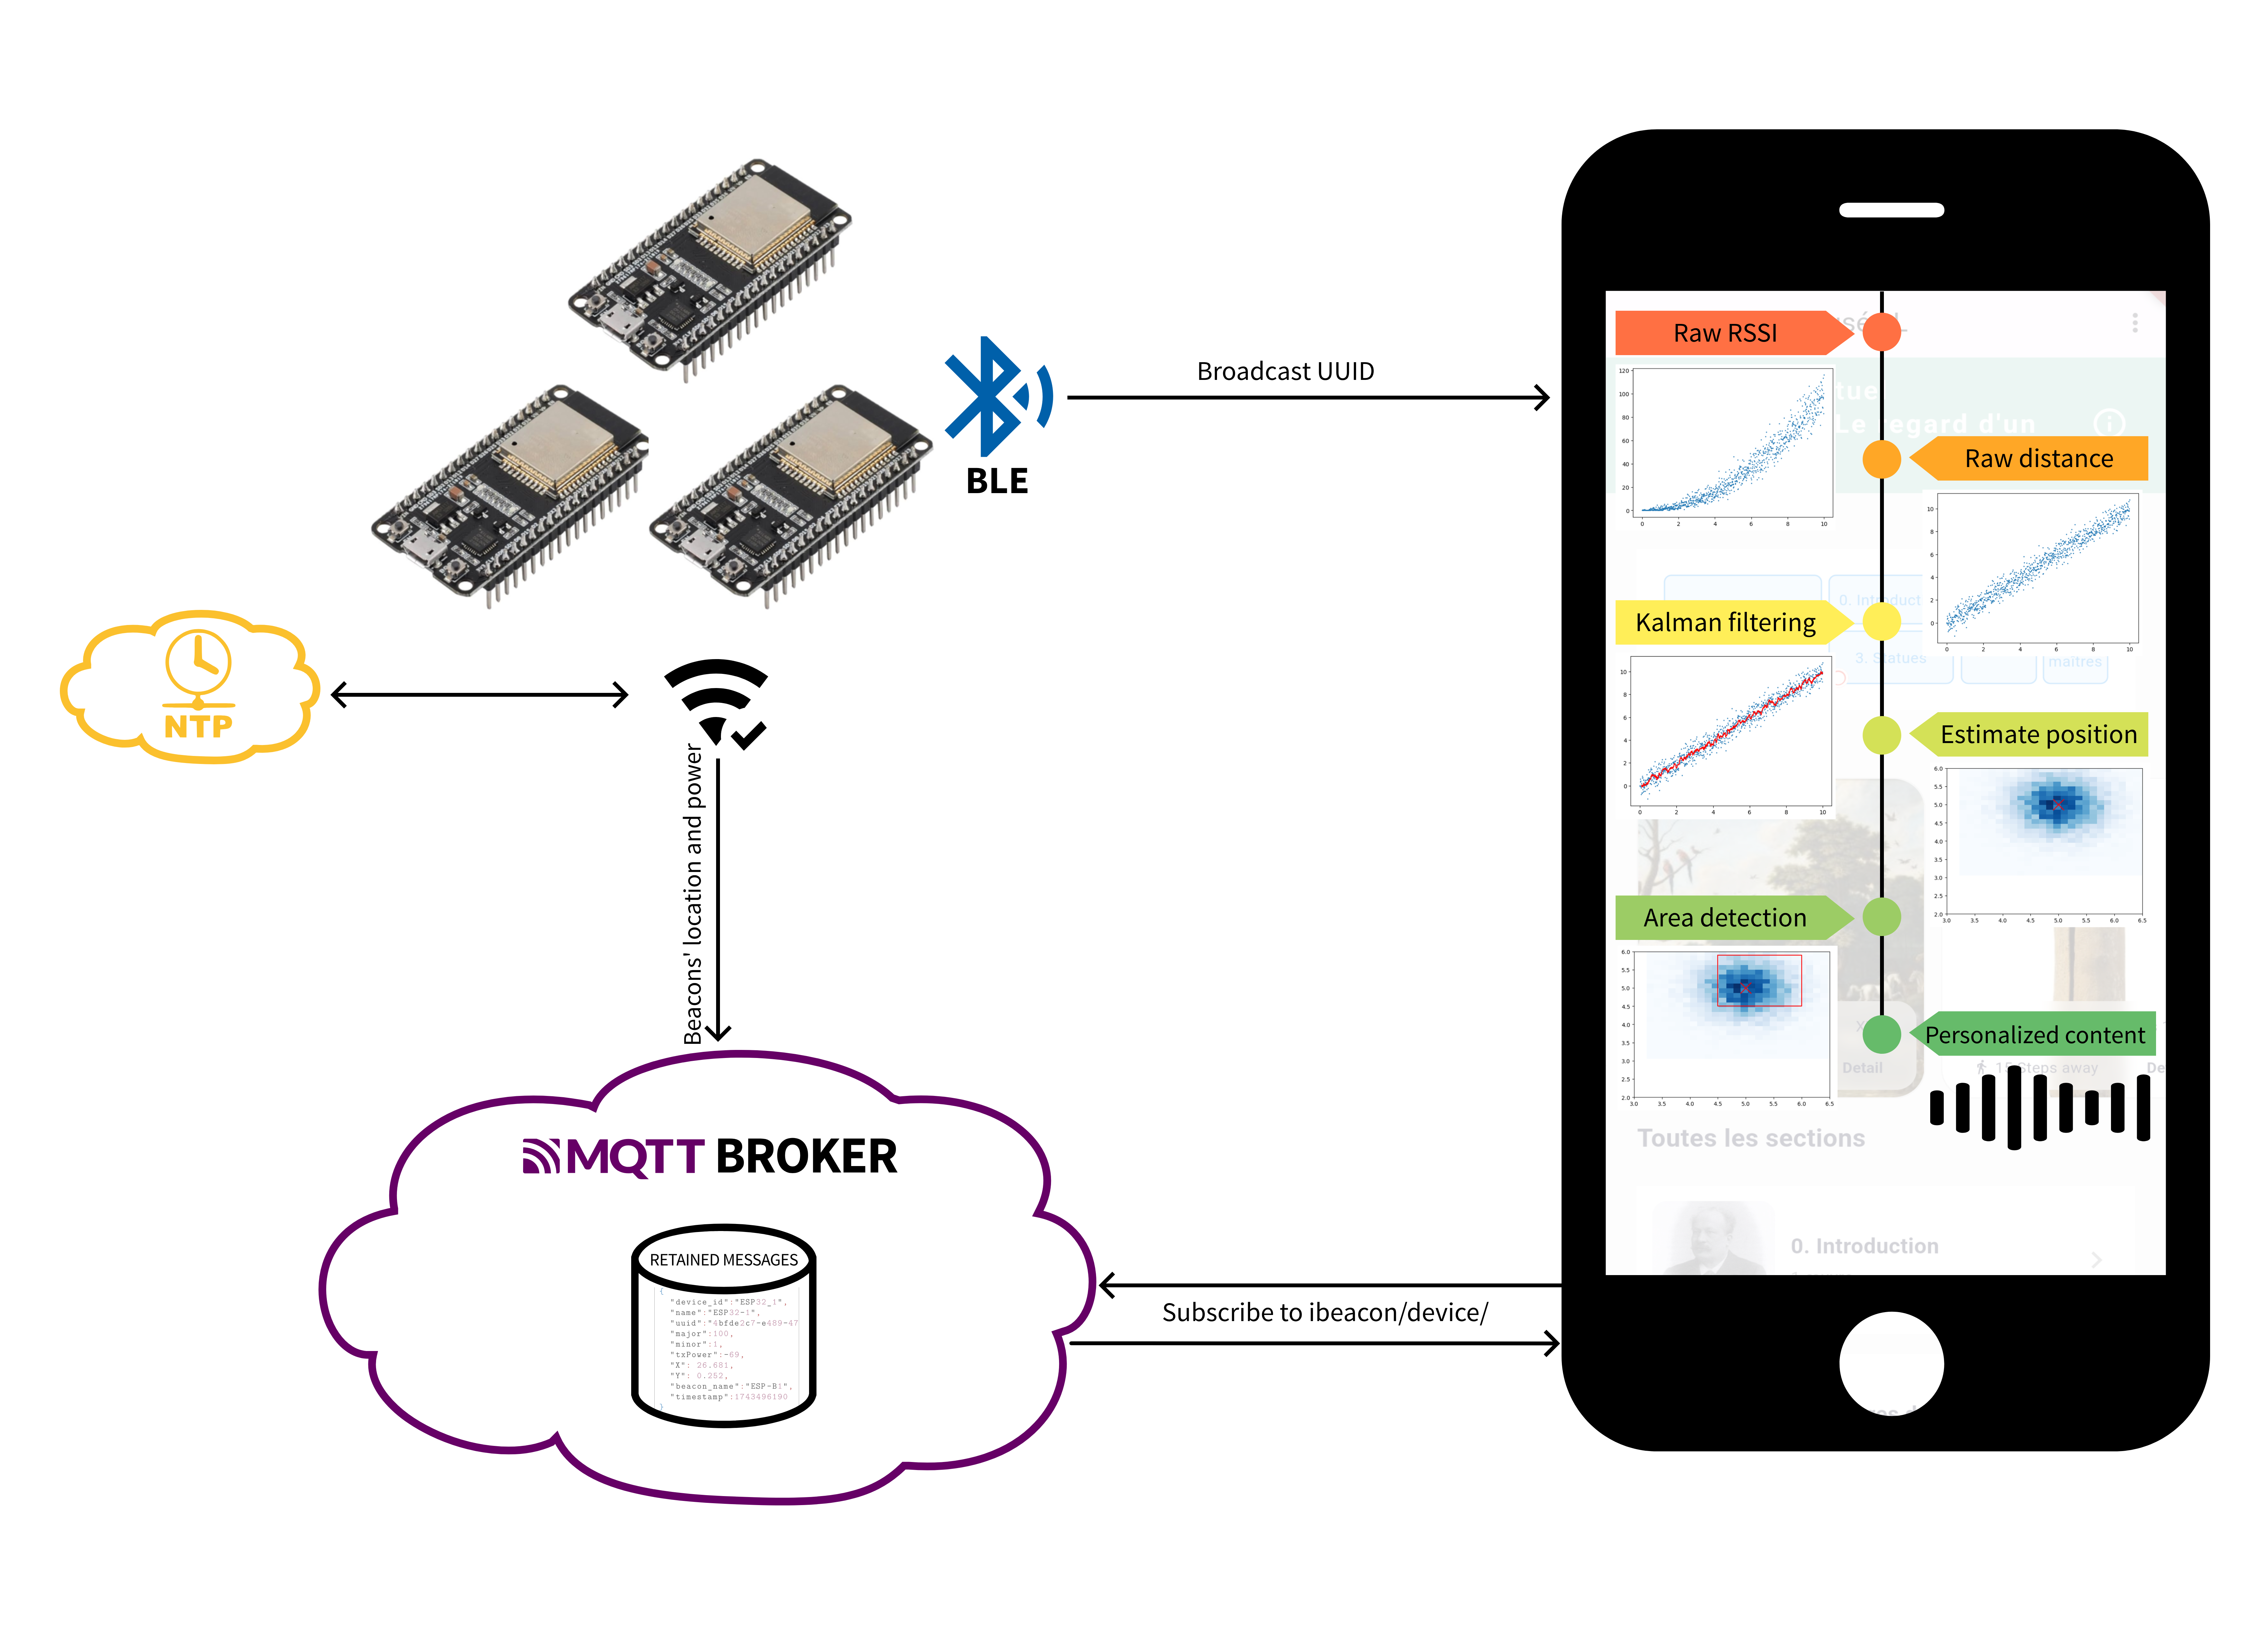
\includegraphics[width=0.9\linewidth]{assets/schema.png}
    \caption{Schema of the full system architecture.}
    \label{fig:schema}
\end{figure}

First, ESP32 devices are used as BLE beacons to broadcast their position. These devices operate by periodically transmitting Bluetooth Low Energy (BLE) signals, ensuring reliable communication with nearby devices. When network access is available, they upload their position data to an MQTT broker, enabling real-time updates across the system.

Second, a smartphone application is developed to receive and process these beacon signals. This application retrieves a list of authorized BLE beacon signatures and uses them to identify and locate nearby ESP32 devices. The application’s design focuses on providing a seamless user experience, with clear and intuitive interfaces for displaying relevant information, and guiding visitors through the museum. It also includes features for audio explanations of areas and art pieces, enhancing the visitor experience by providing context and information about the exhibits.

Third, a cloud MQTT broker facilitates communication between the ESP32 devices and the smartphone application. This decentralized approach eliminates the need for a central server, enhancing the system’s scalability and reducing potential points of failure. Together, these components form a robust and efficient architecture suitable for applications like museum indoor positioning.

\section{ESP32 Beacons}
The ESP32 devices are low-cost, versatile microcontrollers that can be configured to function as BLE beacons. These devices are equipped with a custom firmware that enables them to broadcast their position periodically. When network access is available, they upload their position data to an MQTT broker; otherwise, they operate as standalone beacons, ensuring continuous functionality even in offline scenarios. An illustration of the ESP32 device is shown in \autoref{fig:esp32}.

\begin{figure}
    \centering
    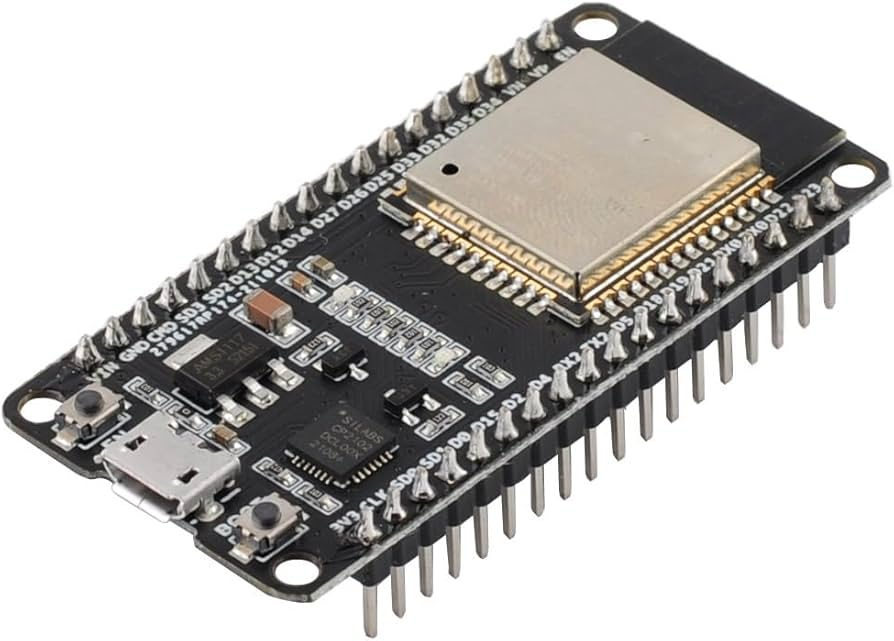
\includegraphics[width=0.5\linewidth]{assets/image-esp32.jpg}
    \caption{Photo of the ESP32}
    \label{fig:esp32}
\end{figure}

The firmware is built in C++, using the standard Arduino library and some popular and bullet-proven packages to handle dedicated critical features such as MQTT communication and BLE management. This choice ensure an efficient firmware while using proven technologies to ensure minimal power consumption and reliable operations even on edge cases. The beacons broadcast at the default frequency of 100ms\footnote{\url{https://reference.arduino.cc/reference/en/libraries/arduinoble/ble.setadvertisinginterval/}}.

A BLE beacon can be uniquely identified using three values: UUID, Major, and Minor. All the beacons used in the system are configured with the same UUID, \texttt{4bfde2c7-e489-47a9-965e-484dae07e8dd}, and major value, \texttt{100}, to ensure that they are recognized as part of the system, as those data are hardcoded both on the ESPs and in the application, to ensure that only the relevant beacons are taken into account. Those values have been arbitrarily chosen and are not relevant to the system's functionality. The minor value is used to differentiate between individual beacons, with each ESP32 device assigned a unique minor value ranging from $1$ to $n$.

The ESP32 have two phases of operation: the initialization phase and the running phase. During the initialization phase, the ESP32 device starts by identifying itself using its internal MAC address to determine its unique minor value and its localization. It then setups and starts its BLE advertising server that will asynchronously broadcast the beacon signal. Broadcasting so early in the setup ensure fast discoverability and efficiency even in case of a failure in another part of the setup as it is the more critical and important part of the system. The device then attempts to connect to a local Wi-Fi network using the credentials provided in the firmware. If the connection is successful, it connects to a predefined NTP server, \texttt{pool.ntp.org}, to retrieve the current time, which is used to timestamp the position data. The device then attempts to connect to the MQTT broker using the provided credentials. 

Once the device is initialized, it enters the running phase, where it continues to broadcast BLE signals. The device also checks for network access every 5 seconds. If the connection is broken, the device will attempt to reconnect to the Wi-Fi network, the NTP server, and the MQTT broker. If the connection is successful, the device will upload its position data to the MQTT broker every 5 seconds. The ESP32 blue LED indicates the current status of the device: it blinks every 50 milliseconds when the device tries to connect to the Wi-Fi network and every 5 seconds when the device is working properly.

\section{Smartphone Application}
The smartphone application is a critical component of the system, responsible for displaying information to the visitor while collecting and processing BLE beacon signals in the background to enhance the visitor experience. It is built using the Flutter framework, which allows for cross-platform development and ensures compatibility with both Android and iOS devices. It also provides a huge collection of packages to handle low-level features of the application, such as BLE management, MQTT communication, data visualization, permissions and audio players, allowing to focus on the application logic and user experience.

The current version of the application contains only the 6th floor of the museum, which is the only one that has been equipped with ESP32 beacons and is analysed in this study. The application is designed to be user-friendly, with a simple and intuitive interface that allows users to easily navigate through the available features while not being forced to use any of them. The home page displays three different sections and is shown in \autoref{fig:app-homepage}. The first one is a map of the floor, with the user's current location indicated by a green dot, the current area with a green background while the others areas are shown with a blue background. Main art-pieces are marked with a red dot. The visitor can click on a specific section to access its content. The second section is a horizontal list of the closest art-pieces, shorted by distance, with current section art-pieces first. Each art-piece is represented by a card containing its name, realization date and rounded distance in steps. A button allows the visitor to access the art-piece page. The third section is a list of all the areas of the floor, with the current area highlighted. Each area is represented by a card containing its name, one of the art-pieces and the amount of art-pieces presents in the area. The user can click on a specific area to access its content. 

The area page shown in \autoref{fig:app-area} displays the list of art-pieces in the area, with more information than the home page. It also provides an audio explanation of the area, which is played automatically when the visitor enters it. The visitor can always decide to stop the audio playback, or to listen to the audio explanation of another area. If the user move from an area to another during the audio playback, the audio will not be interrupted, but the audio of the new area will be played when the previous one is finished. The audio files are stored locally in the application. If the visitor is still in the area when the audio playback is finished, the audio will stop, and the user has the ability to play it again, or to listen to the audio of a specific art-piece for more information. The audio files are played using the native audio player of the smartphone, allowing the visitor to listen to them while navigating through the application or even with the device turned off. The area page also contains a button to access the home page.

The art-piece page shown in \autoref{fig:app-art-piece} displays a picture of the art-piece and all the available information. If the art-piece contains an audio explanation, the user can listen to it by clicking on the play button. Art-piece specific audio will never be played automatically as the wish to get more information about an art-piece depends on the visitor. The audio file works the same way as the area audio file, allowing the visitor to listen to it while navigating through the application, or to change area without interrupting the audio playback. The art-piece page also contains a button to access the area page.

The current content of the application is limited to demonstration purposes, with only a few art-pieces available. The application is designed to be easily extensible, allowing for the addition of new content and features in the future. It also contains a top bar menu to access the debug and experiment pages. The debug page contains a map of the floor with the beacons' location, the estimated distance to each beacon, and the current location of the user. The experiment page allows recording data following the instructions provided in \autoref{chap:methodology}.

\begin{figure}[h]
    \centering
    \begin{subfigure}[b]{0.33\linewidth}
        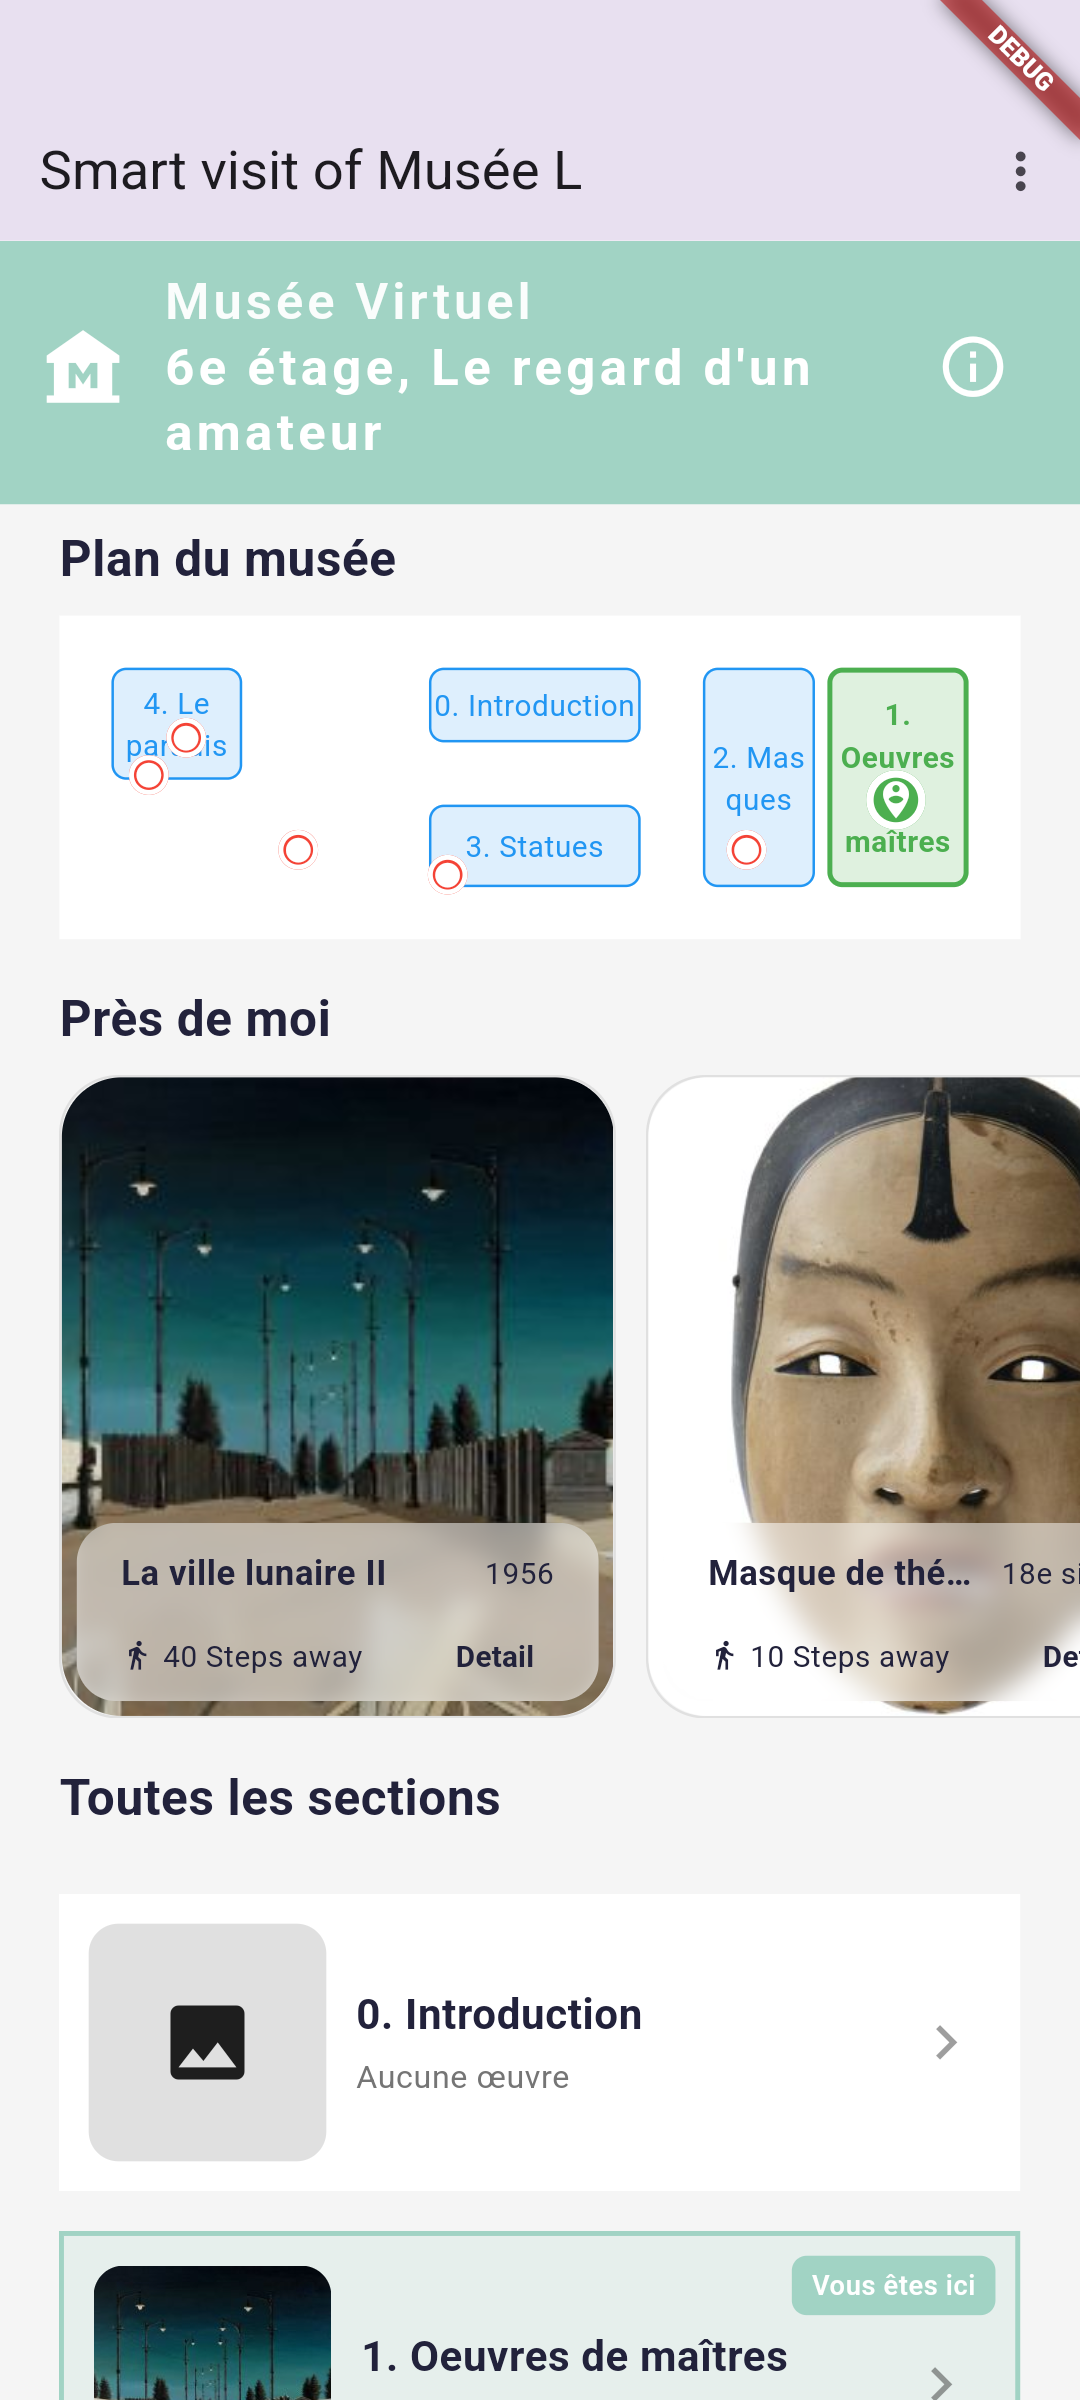
\includegraphics[width=\linewidth]{assets/application-homepage-top.png}
        \caption{Top of the home page}
        \label{fig:app-homepage-top}
    \end{subfigure}
    \hspace{3em} % or another fixed space
    \begin{subfigure}[b]{0.33\linewidth}
        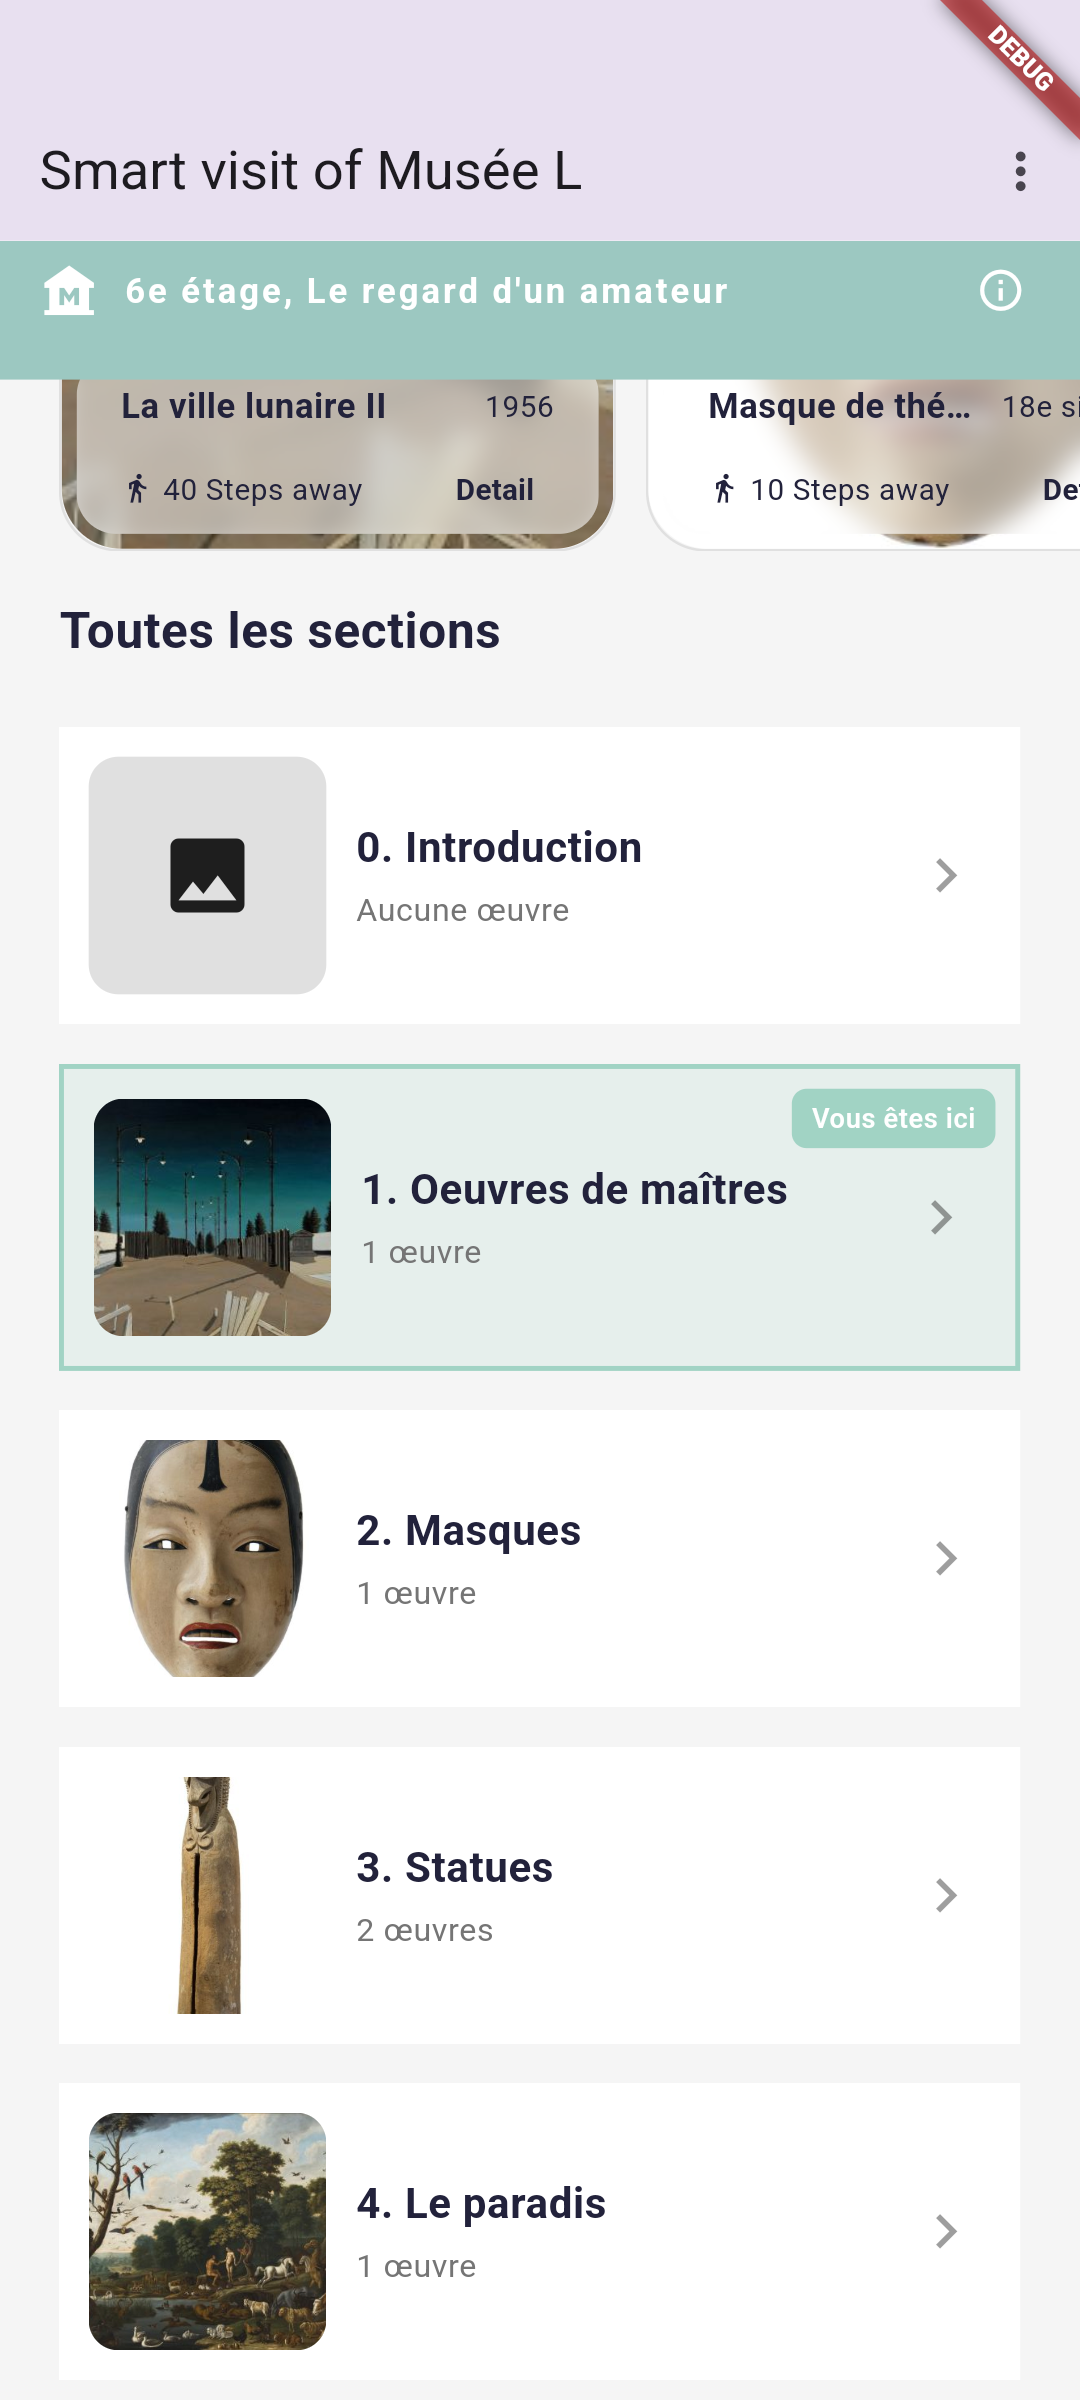
\includegraphics[width=\linewidth]{assets/application-homepage-bottom.png}
        \caption{Bottom of the home page}
        \label{fig:app-homepage-bottom}
    \end{subfigure}
    \caption{Screenshots of the home page: top (left) and bottom (right).}
    \label{fig:app-homepage}
\end{figure}

\begin{figure}[h]
    \centering
    \begin{subfigure}[b]{0.33\linewidth}
        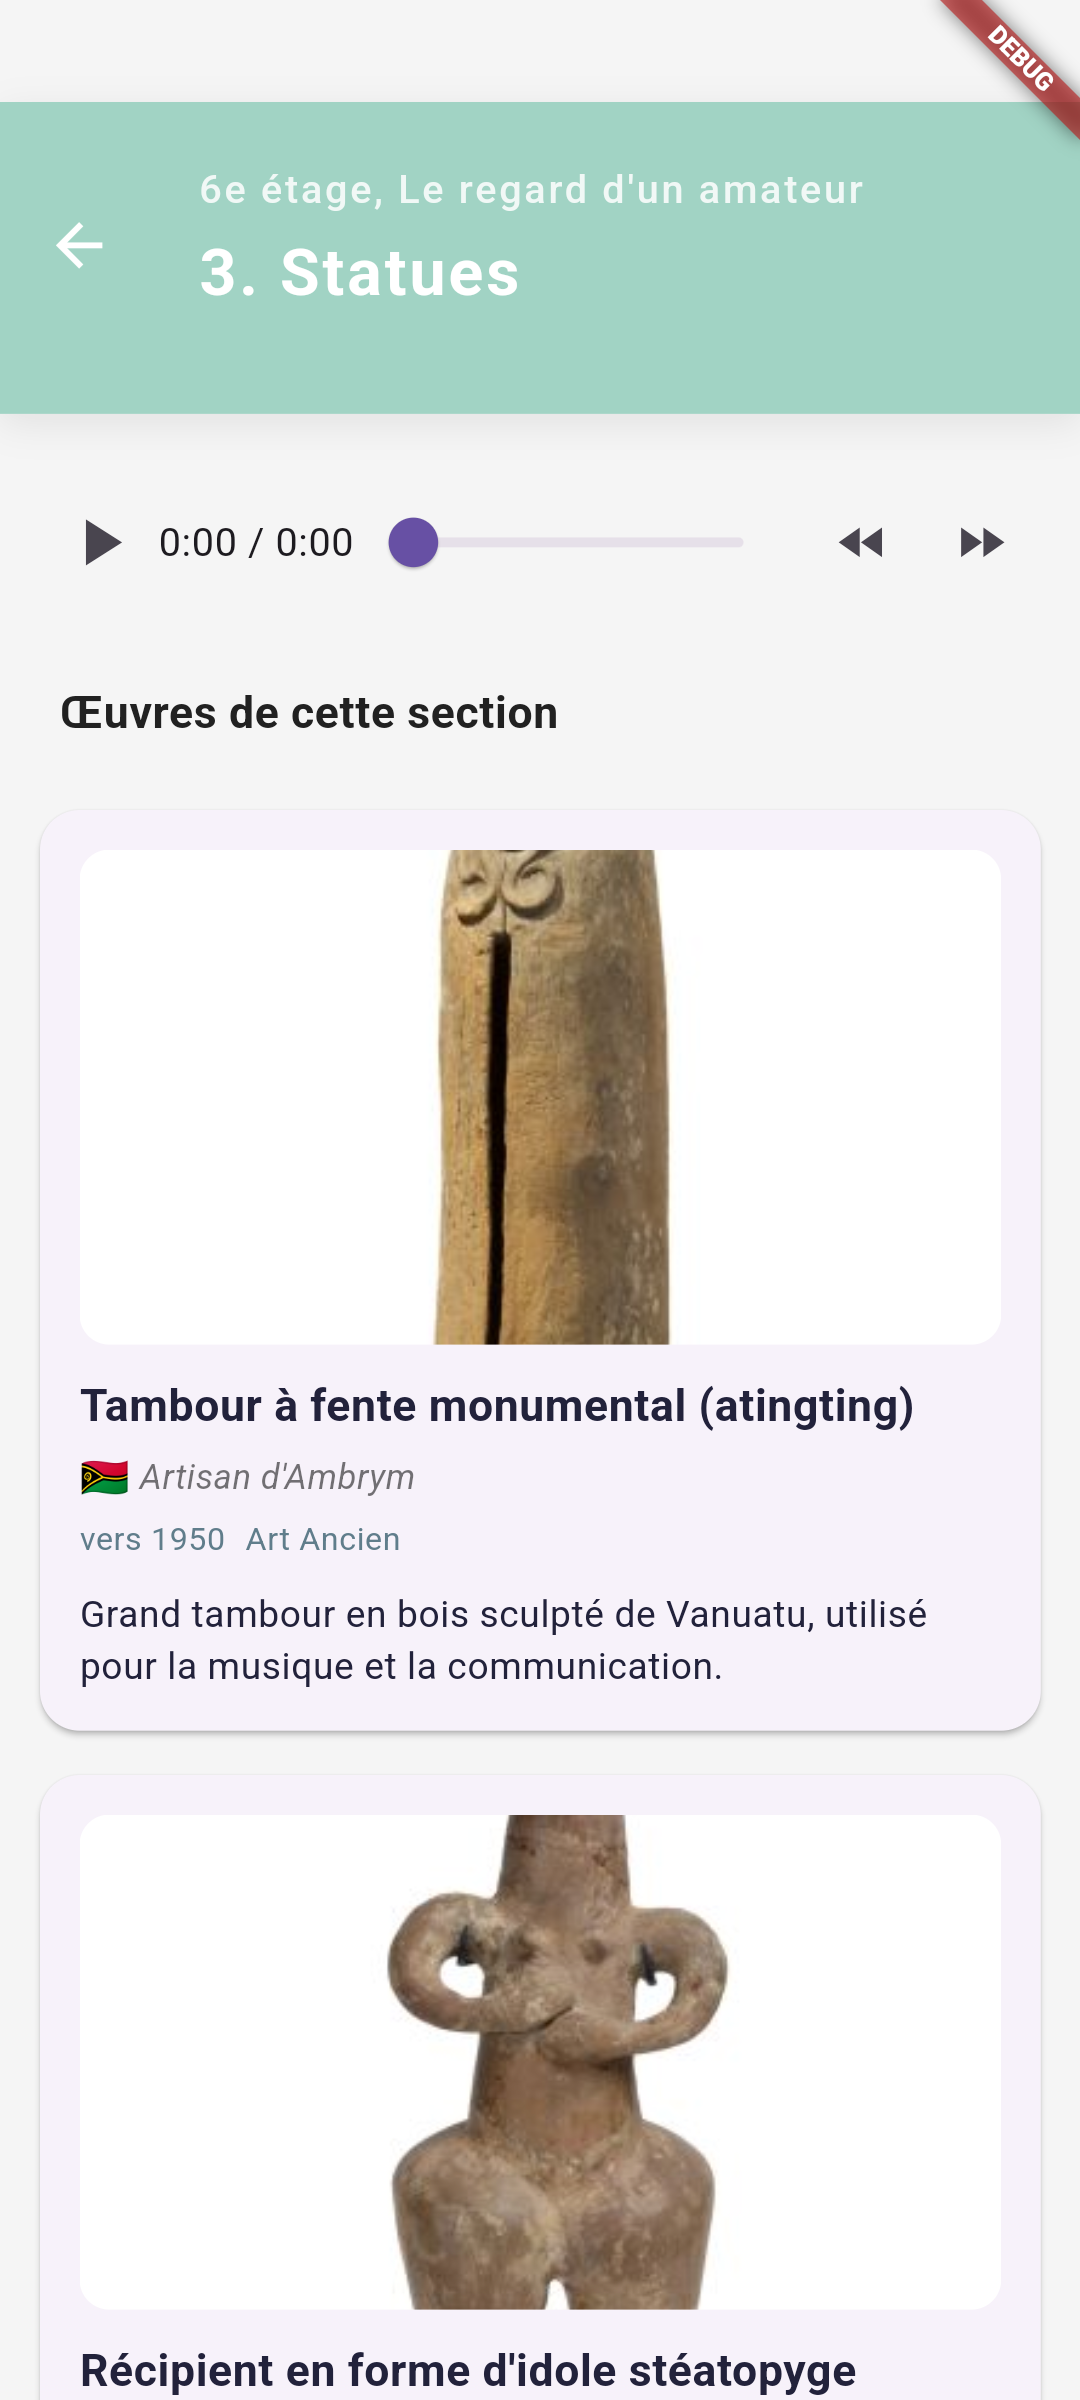
\includegraphics[width=\linewidth]{assets/application-area.png}
        \caption{Area page}
        \label{fig:app-area}
    \end{subfigure}
    \hspace{3em} % or another fixed space
    \begin{subfigure}[b]{0.33\linewidth}
        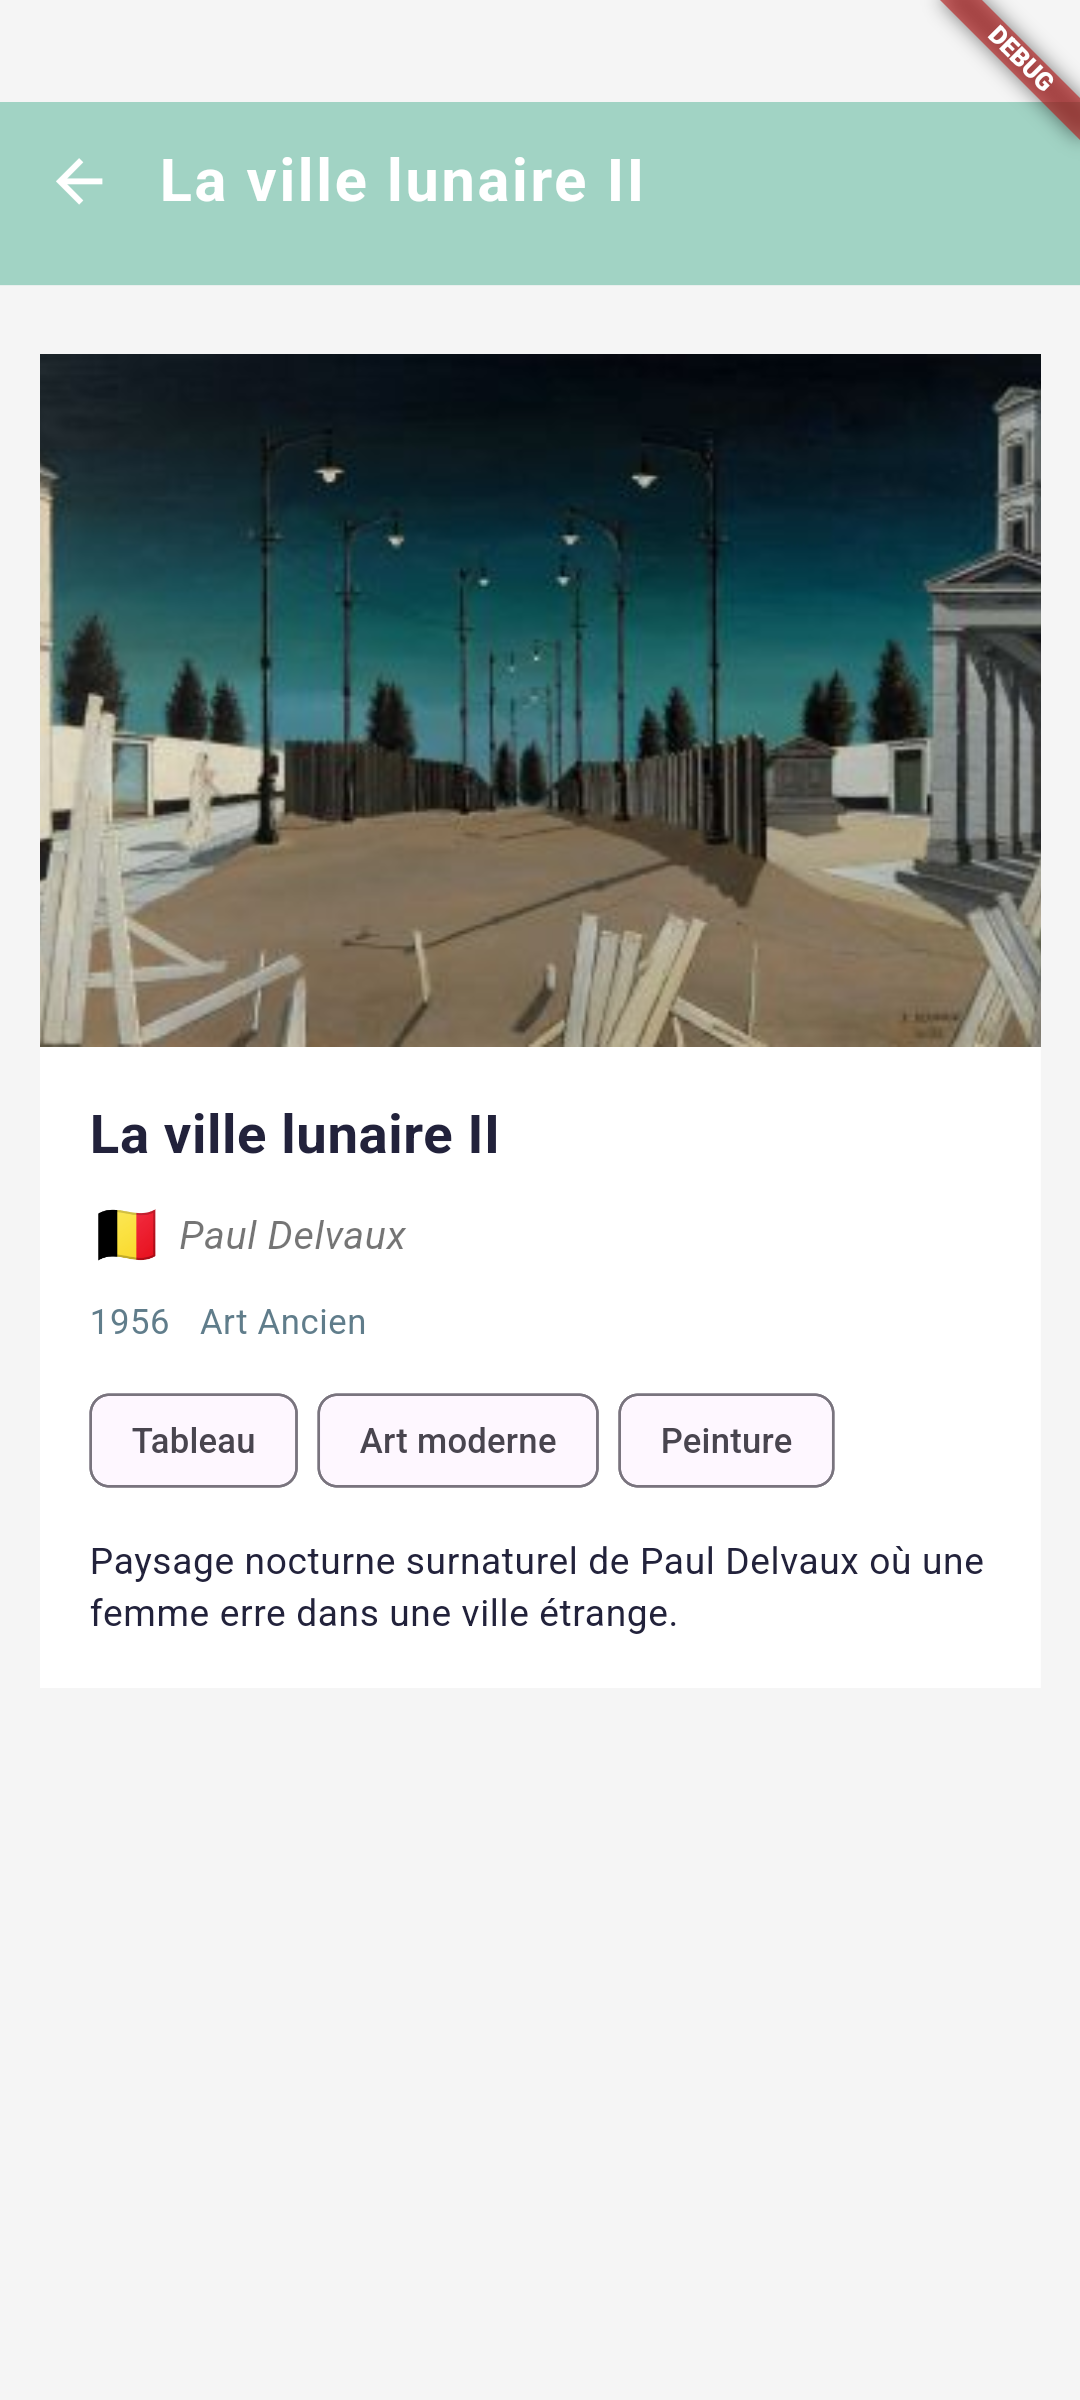
\includegraphics[width=\linewidth]{assets/application-art-piece.png}
        \caption{Art piece page}
        \label{fig:app-art-piece}
    \end{subfigure}
    \caption{Screenshots of the area page (left) and art piece page (right).}
    \label{fig:app-area-piece}
\end{figure}

The background process retrieves the list of authorized BLE beacon signatures and use them to identify and locate nearby ESP32 devices. This process involves scanning for BLE signals, filtering out unauthorized beacons, and calculating the user’s distance relative to the detected devices, and then use those data to determine the user's position. Finally, the change of user position is sent to the front-end to update the map, the list of closest art-pieces, and detect when the user changes area.

The core localization logic in the application is designed to robustly estimate the user's position using signals from multiple BLE beacons. For each beacon, the application maintains a filtered estimate of distance, leveraging a Kalman filter to smooth out the inherent noise in RSSI measurements. At each update, the system selects up to six beacons with the lowest estimated distances, ensuring that only the most relevant and reliable signals are used for position calculation.

To determine the user's location, the algorithm considers all possible combinations of three beacons among the selected set. For each trio, it computes a weighted centroid, where the influence of each beacon is adjusted according to the relative distances. The quality of each triangle formed by the beacon positions is also assessed, favouring well-shaped, non-degenerate triangles to improve accuracy. The final estimated position is then calculated as a weighted average of all candidate positions, with higher-quality triangles contributing more to the result. This approach balances robustness and precision, allowing the application to provide real-time, reliable localization even in the presence of signal fluctuations and environmental noise.

To determine the user's location, the algorithm examines all possible combinations of three beacons from the selected set. Each group of three beacons defines a triangle, and for each triangle, the algorithm computes a candidate position using a geometric centroid approach. To assess the reliability of each triangle, a quality score is computed based on its shape. The area of the triangle count for 70\% of the score, with bigger triangles being preferred as they are less likely to be affected by noise or interference. The angles of the triangle contribute the remaining 30\%, where each angle between 30° and 120° is considered optimal, with angles outside this range penalized. This ensures that the algorithm favours well-shaped triangles, which are more likely to yield accurate position estimates. The final estimated position is then calculated as a weighted average of all candidate positions.

The application is built with privacy and security as core design principles, ensuring that user data remains completely protected at all times. It follows a strict privacy-by-design approach, meaning no personal information is ever collected, transmitted, or stored. The only form of communication is a passive subscription to an MQTT broker, allowing the application to receive positional data from ESP32 devices without sending any data in return. This one-way, receive-only mechanism eliminates the risk of data leaks or misuse, reinforcing the application's commitment to user confidentiality. 

Security is equally prioritized through a decentralized architecture that avoids centralized data storage or user identification. By using lightweight and secure communication protocols, and eliminating unnecessary data exchange, the system minimizes exposure to potential vulnerabilities. This secure-by-design approach ensures that all operational processes inherently protect user information, making the application not only efficient but also inherently safe and trustworthy. 

\section{MQTT Broker}
	The MQTT broker serves as the communication backbone of the system, enabling seamless data exchange between ESP32 devices and the smartphone application. ESP32 devices upload their position data to the broker whenever network access is available. This data is then relayed in real-time to the smartphone application, ensuring that users receive up-to-date information without noticeable delays. Those position data are published as retained message, ensuring that the smartphone application receives the last known position of the ESP32 devices even if they are not connected to the MQTT broker. The data are published on the topic \texttt{ibeacon/devices/<UUID>\_<MAJOR>\_<MINOR>}. A typical payload of the position data is shown in \autoref{lst:payload}.

\begin{lstlisting}[language=json, caption={Payload of the position data}, label={lst:payload}]
{
  "device_id":"ESP32_1",
  "name":"ESP32-1",
  "uuid":"4bfde2c7-e489-47a9-965e-484dae07e8dd",
  "major":100,
  "minor":1,
  "txPower":-69,
  "X": 26.681,
  "Y": 0.252,
  "beacon_name":"ESP-B1",
  "timestamp":1743496190
}
\end{lstlisting}

The use of a cloud MQTT broker offers several advantages. First, it eliminates the need for a managed server, enhancing the system’s scalability and reducing potential points of failure, as the system is provider-agnostic. Second, it supports asynchronous communication, allowing devices to operate independently while still sharing data efficiently. Finally, the broker’s lightweight protocol is well-suited for low-power devices like the ESP32, ensuring minimal impact on battery life.

This decentralized approach not only improves system reliability but also simplifies maintenance and upgrades. By leveraging the MQTT broker, the system achieves a high level of flexibility and efficiency, making it suitable for a wide range of applications.

